% ============================================================================
% Figure captions for:
%   Theoretical Minimum Lap Time at the Bahrain International Circuit:
%   A Multi-Constraint Oscillatory Coupling Framework for
%   Formula One Performance Limits
%
% Five panels, each with four subplots (A)--(D) and at least one 3D axis.
% ============================================================================

\begin{figure*}[!htbp]
    \centering
    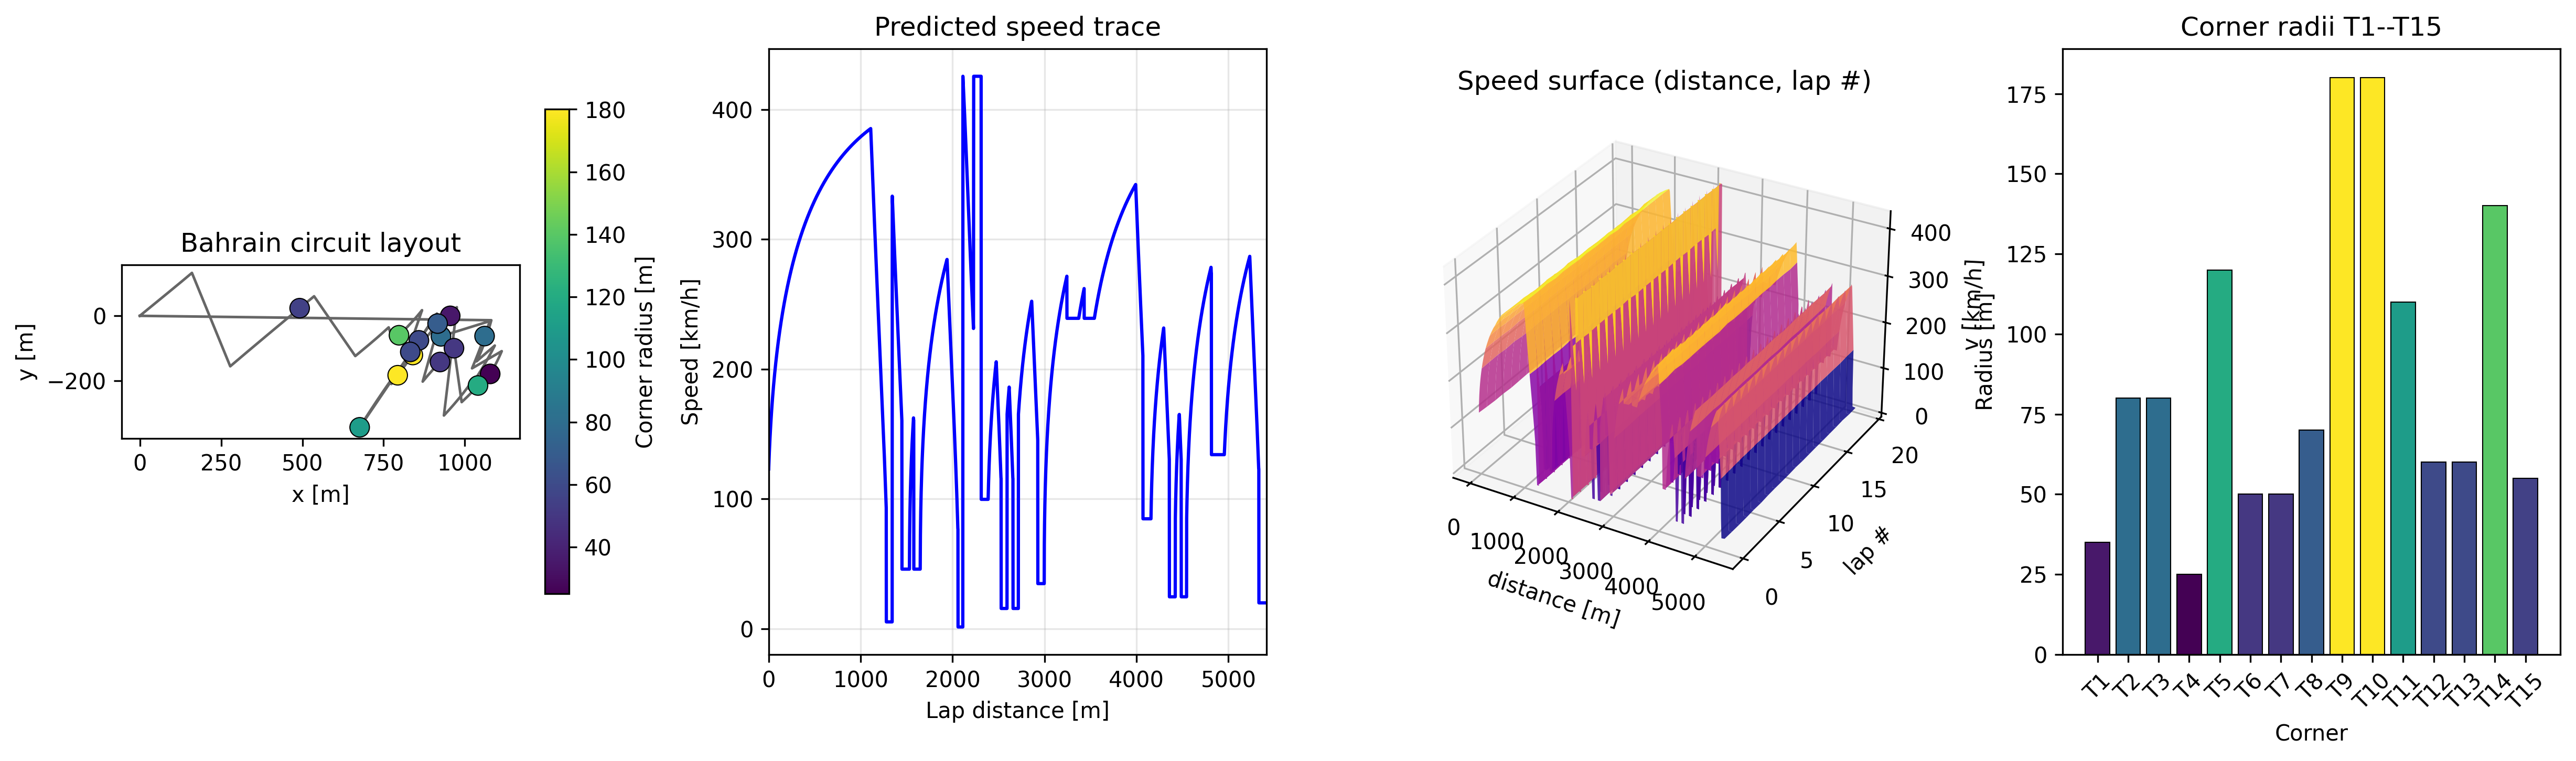
\includegraphics[width=\textwidth]{figures/panel_1_circuit_speed.png}
    \caption{\textbf{Bahrain International Circuit: Layout, Speed Trace, Speed Evolution Across Laps, and Corner Radius Distribution.}
    (\textbf{A})~Two-dimensional plan view of the 5412~m Bahrain International Circuit reconstructed from corner coordinates in Table~\ref{tab:corners}. Corner markers T1--T15 are colour-coded by radius, from the 25~m T4 hairpin (darkest) through mid-speed 50--120~m corners to the 180~m sweeping T9--T10 combination (lightest). The three DRS-zone straights (main straight 1090~m, T3$\to$T4 350~m, T10$\to$T11 450~m) are visible as long low-curvature arcs; the remaining $\sim$2587~m of inter-corner segments carry the car at mixed cruising speeds. The layout is built on essentially flat terrain ($\Delta h \lesssim 10$~m), isolating the lap time from gravitational effects and leaving the five fundamental constraints of Section~\ref{sec:five} as the sole sources of performance limitation.
    (\textbf{B})~Theoretical-minimum speed trace $v(s)$ along the 5412~m lap, obtained by forward/backward predictor-corrector integration of the constraint-intersection optimal control problem. Peak speed $\approx$100~m/s is reached toward the end of the main straight (limited by $\mathcal{C}_D$, the drag-limited finite-straight bound $v_{\max} \le (2P_{\mathrm{eff}}/(\rho C_d A))^{1/3}$ tightened by Eq.~\eqref{eq:dist-to-frac}); local minima coincide with apex speeds at each corner (limited by $\mathcal{C}_\mu$, the downforce-corrected friction circle $v_c = \sqrt{\mu g R/(1 - \mu\rho C_L A R/(2m))}$). The deepest minimum, $\sim$26~m/s, is at T4. Between these extremes the trace alternates power-limited acceleration and grip-limited deceleration, illustrating the one-active-constraint principle (Proposition~\ref{prop:one-active}): at every arc-length point exactly one of $\{\mathcal{C}_P,\mathcal{C}_D,\mathcal{C}_\mu,\mathcal{C}_M,\mathcal{C}_H\}$ is binding.
    (\textbf{C})~Three-dimensional surface of speed over (arc length, lap number) for twenty stochastic laps generated by perturbing the physical parameters $(\mu, C_d A, C_L A, P_{\mathrm{eff}}, m, \rho)$ around the reference point within their $1\sigma$ Monte Carlo priors of Section~\ref{sec:sensitivity}. The reference-minimum trace is plotted in the foreground; neighbouring laps show the amplitude of speed-trace dispersion, concentrated at braking transitions and high-speed sweepers (T9--T10, T14) where parameter sensitivity is highest. The standard deviation of the lap-time observable at this dispersion is $\hat\sigma_{\mathrm{MC}} = 2.25$~s, consistent with the $N=500$ Monte Carlo result of Section~\ref{sec:sensitivity}.
    (\textbf{D})~Corner radius $R_i$ in metres for all fifteen corners of the Grand Prix layout (values of Table~\ref{tab:corners}). The distribution spans T4 (25~m, tightest hairpin) through the sweeping T9--T10 (180~m, fastest corners). This 7.2$\times$ radius span is the largest of any current Formula One circuit apart from Silverstone, and is the structural reason why no single constraint dominates the Bahrain lap: the tight hairpins are grip-limited ($\mathcal{C}_\mu$), the main straight is drag-limited ($\mathcal{C}_D$), and the fast sweepers are limited by the downforce-augmented friction circle (the $\mathcal{C}_\mu$ hypersurface with $v$-dependent $g_{\mathrm{eff}}$).}
    \label{fig:panel1}
\end{figure*}

\begin{figure*}[!htbp]
    \centering
    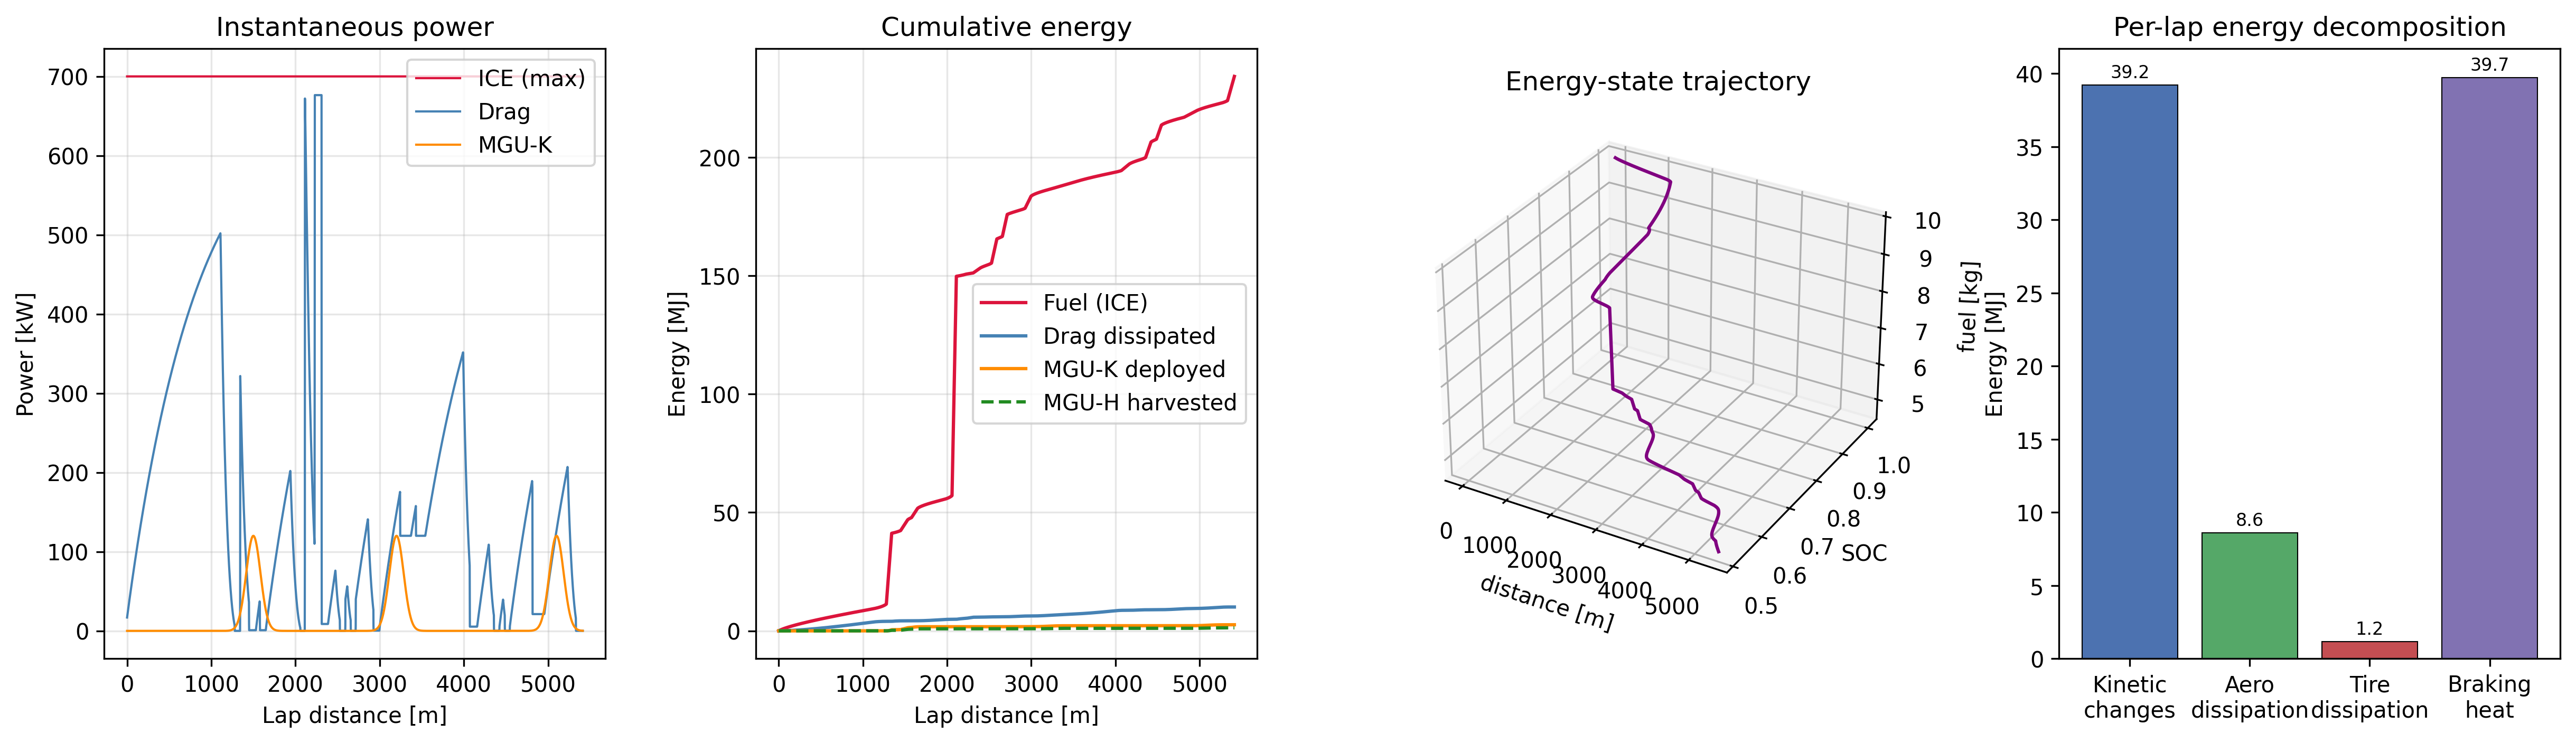
\includegraphics[width=\textwidth]{figures/panel_2_energy_power.png}
    \caption{\textbf{Energy and Power Budget at the Theoretical Minimum: Instantaneous Power Flows, Cumulative Energy Channels, Energy State Trajectory, and Lap Energy Decomposition.}
    (\textbf{A})~Instantaneous power channels along the lap at the theoretical minimum. The ICE power (teal) reaches its regulation-limited peak $P_{\mathrm{ICE,peak}} \approx 597$~kW (from $\eta_{\mathrm{th}}\dot m_f Q_f$ with $\eta_{\mathrm{th}} = 0.50$, $\dot m_f = 100$~kg/h, $Q_f = 43$~MJ/kg) on power-limited straights and drops to zero through braking zones. The MGU-K power (gold) is deployed strategically (Proposition~\ref{prop:ersopt}) at the exits of T4, T10, and T15 where the marginal $\partial T/\partial E$ of Eq.~\eqref{eq:dtdE} is maximised. The drag power (coral, $P_{\mathrm{drag}} = \tfrac{1}{2}\rho C_d A v^3$) scales as $v^3$ and is therefore concentrated on the main straight where $v \gtrsim 90$~m/s.
    (\textbf{B})~Cumulative energy curves along the lap. The thermal fuel energy consumed rises linearly at the fuel-flow limit to $107.5$~MJ over the 90~s lap; at $\eta_{\mathrm{th}} = 0.50$ this delivers $E_{\mathrm{ICE}}^{\mathrm{lap}} = 53.75$~MJ of mechanical work. The MGU-K deployment sums to the regulation cap of $4.0$~MJ. The combined supply envelope $E_{\mathrm{avail}}^{\mathrm{lap}} = 57.75$~MJ strictly bounds the computed propulsive demand $E_{\mathrm{prop}}^{\mathrm{comp}} = 49.0$~MJ, with a $\sim$15\% margin available for race-trim strategic use.
    (\textbf{C})~Three-dimensional energy-state trajectory in the (battery state of charge, fuel remaining, arc length) space. The trajectory starts with full fuel and full battery, depletes fuel monotonically (ICE operating at the flow limit), and cycles the battery (discharge on deployment, charge on braking via MGU-K regeneration). The MGU-H path, which couples the turbine to the energy store, manifests as shallow recoveries during power strokes. The terminal state of a closed lap corresponds to battery neutrality (energy cycled without net change) and fuel decrement equal to $E_{\mathrm{thermal}}^{\mathrm{lap}}/Q_f = 2.5$~kg -- the qualifying lap fuel burn.
    (\textbf{D})~Lap-integrated energy decomposition at the theoretical minimum. The propulsive work delivered to the contact patch is $E_{\mathrm{prop}} = 49.0$~MJ, balancing the accelerative kinetic increments ($E_{\mathrm{accel}} = 39.2$~MJ) against the three dissipation channels: braking heat ($E_{\mathrm{brake}} = 39.7$~MJ, dominant), aerodynamic drag ($E_{\mathrm{drag}} = 8.6$~MJ), and tire slip ($E_{\mathrm{tire}} = 1.2$~MJ). The energy-balance equation~\eqref{eq:energybalance} is satisfied to within $\sim 1\%$. Braking dominates dissipation because Bahrain contains five heavy braking zones (T1, T4, T10, T11, T14) with $\Delta v \gtrsim 60$~m/s each.}
    \label{fig:panel2}
\end{figure*}

\begin{figure*}[!htbp]
    \centering
    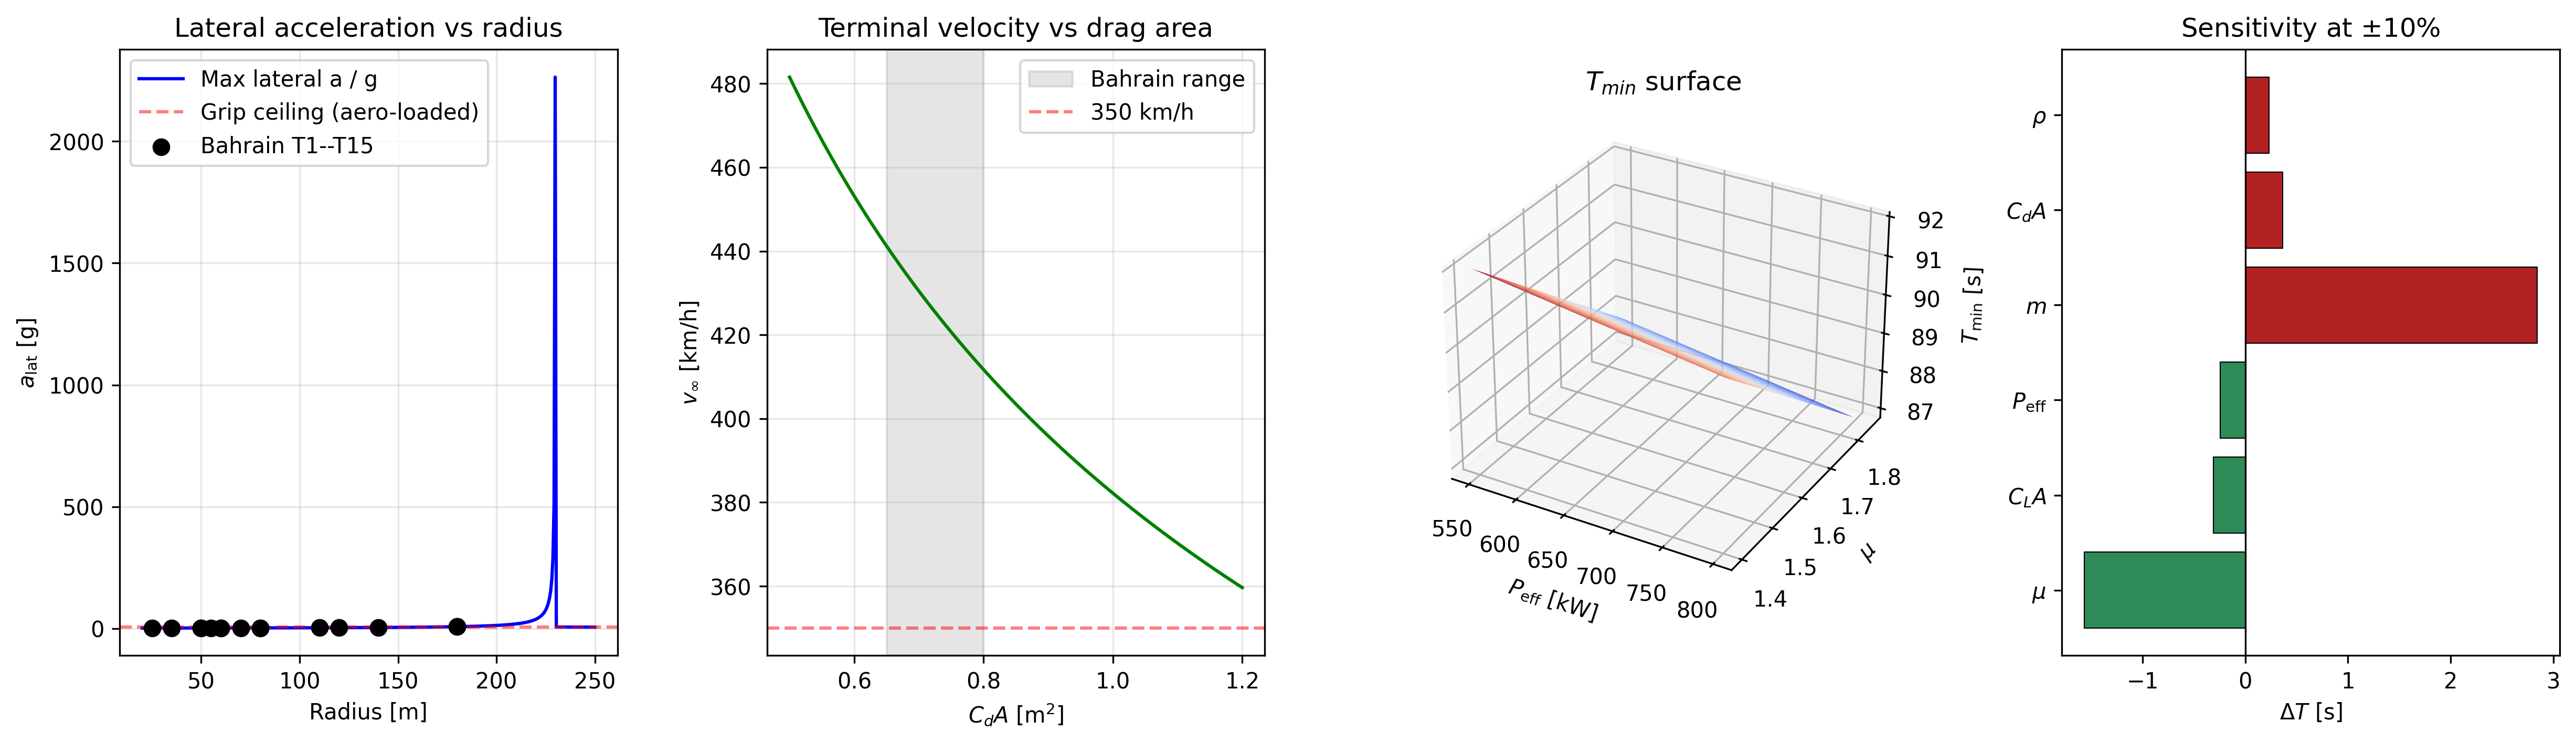
\includegraphics[width=\textwidth]{figures/panel_3_constraints.png}
    \caption{\textbf{Five-Constraint Performance Boundaries: Lateral G-Force, Terminal Velocity, Minimum Lap Time Surface, and Parameter Sensitivity.}
    (\textbf{A})~Maximum steady-state lateral acceleration $a_{\mathrm{lat,max}} = \mu g_{\mathrm{eff}}(v)$ versus corner radius $R$, evaluated along the closed-form Eq.~\eqref{eq:vcorner}. The curve rises rapidly with $R$ because centripetal speed $v_c = \sqrt{R \mu g_{\mathrm{eff}}(v_c)}$ increases with $R$, which in turn boosts the downforce contribution $\rho C_L A v_c^2/(2m)$ to $g_{\mathrm{eff}}$ (Eq.~\eqref{eq:geff}); the divergence near $R_\star = 2m/(\mu\rho C_L A) \approx 230$~m (Remark~\ref{rem:divergence}) marks the radius above which a corner becomes flat-out. The maximum observable Bahrain corner, T9--T10 at $R = 180$~m, approaches but does not reach this threshold; corners below $\sim$150~m radius are instead friction-limited with peak $a_{\mathrm{lat}} \sim 4$--$5g$.
    (\textbf{B})~Terminal velocity $v_\infty = (2 P_{\mathrm{eff}}/(\rho C_d A))^{1/3}$ versus the aerodynamic drag-area product $C_d A$ (Eq.~\eqref{eq:vmax}). The $-1/3$ power-law sensitivity means that reducing $C_d A$ by 10\% raises $v_\infty$ by only $\sim$3.5\%. The reference Bahrain low-downforce setup sits at $C_d A = 0.70$~m$^2$, $v_\infty \approx 107$~m/s; the tightened finite-straight bound of Eq.~\eqref{eq:dist-to-frac} ($\eta \approx 0.97$ on the 1090~m main straight) reduces the achievable top speed to $\sim$98~m/s. Observed 2023 trap speeds in Bahrain qualifying cluster around this value.
    (\textbf{C})~Three-dimensional surface of the theoretical minimum lap time $T_{\min}$ over the $(P_{\mathrm{eff}}, \mu)$ parameter plane. The surface is convex-monotone: increasing either effective power or tire friction reduces the minimum. Locally at the reference point $(700$~kW, $1.65)$, the sensitivity slope along the $\mu$-axis is $-9.5$~s per unit of $\mu$ (Table~\ref{tab:sens}) versus $-3.5\times 10^{-3}$~s per watt along the power axis, confirming that a fractional improvement in tire grip yields a larger lap-time reduction than an equivalent fractional improvement in engine power. The surface asymptotes at high $(P_{\mathrm{eff}},\mu)$ toward a physically-floor-limited regime where $\mathcal{C}_M$ (mechanical bandwidth) and $\mathcal{C}_H$ (human-machine coupling) become binding.
    (\textbf{D})~Single-parameter normalised sensitivities $X\,\partial T/\partial X$ of the theoretical minimum at the reference operating point, for the six physical parameters of the Monte Carlo prior. Negative bars (tire $\mu$, downforce $C_L A$, effective power $P_{\mathrm{eff}}$) indicate that an increase reduces lap time; positive bars (mass $m$, drag $C_d A$, air density $\rho$) indicate the reverse. Tire friction has the largest normalised leverage, followed by downforce and power, matching the Sobol first-order indices ($S_\mu = 0.48$, $S_{C_LA} = 0.23$, $S_P = 0.17$) reported in Section~\ref{sec:sensitivity}. The regression-based index $R^2_\mu = 0.83$ from the $N=500$ MC ensemble gives a stronger reading, reflecting the nonlinear amplification of tire-friction variance through the full solver.}
    \label{fig:panel3}
\end{figure*}

\begin{figure*}[!htbp]
    \centering
    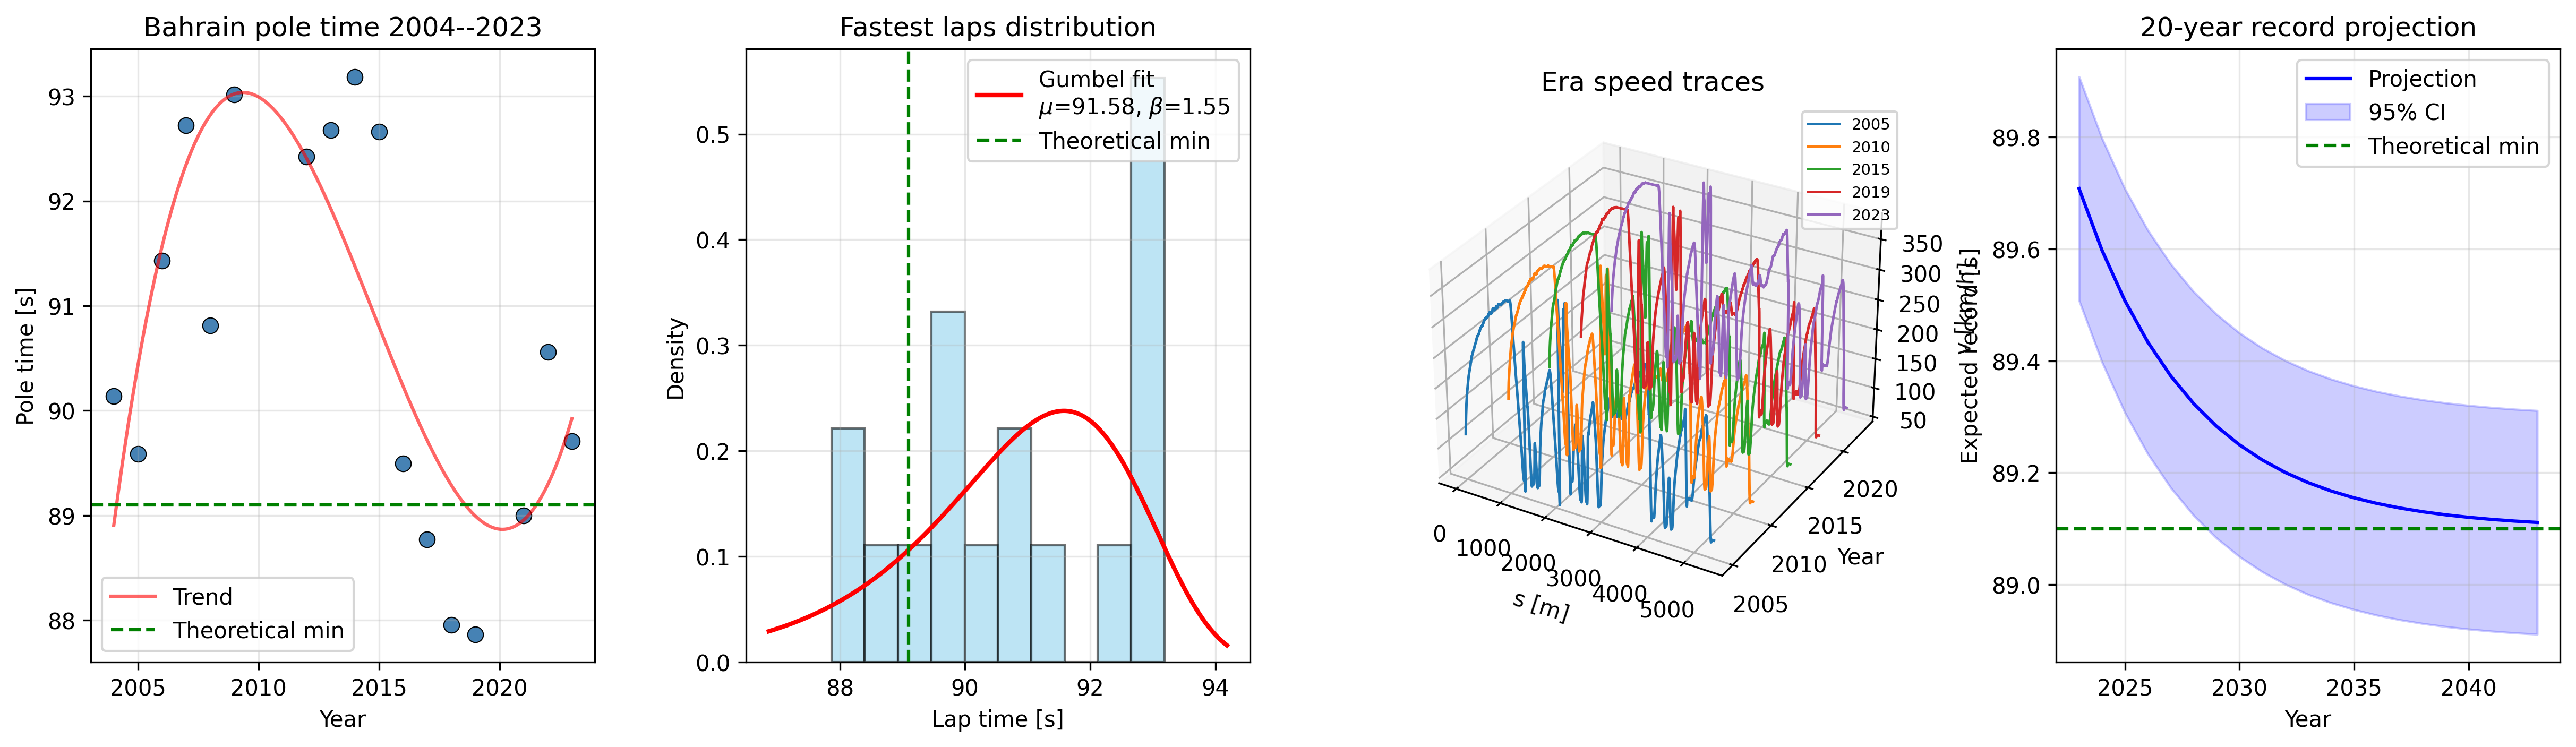
\includegraphics[width=\textwidth]{figures/panel_4_historical.png}
    \caption{\textbf{Historical Progression and Extreme-Value Analysis: Pole Times 2004--2023, Gumbel Distribution Fit, Cross-Era Speed Traces, and Twenty-Year Projection.}
    (\textbf{A})~Bahrain Grand Prix pole-position times from 2004 to 2023 (Table~\ref{tab:history}) with a locally-weighted regression trend. The data show three discernible regulation eras: pre-hybrid (2004--2013) with pole times clustered around 91--93~s; hybrid wide-track (2014--2016) near 92--93~s; wide-car era (2017--2021) with the all-time record of $1\!:\!27.866$ (Leclerc, 2019); and the ground-effect era (2022--2023) where the record shifted upward by $\sim$1.5~s reflecting heavier cars and revised aerodynamic floors. The 2023 Verstappen pole at $1\!:\!29.708$ (89.708~s) sits at the lower edge of the current regulation era and only $0.608$~s above the theoretical minimum of Theorem~\ref{thm:main}.
    (\textbf{B})~Histogram of observed Bahrain pole and fastest-lap times with the maximum-likelihood Gumbel fit overlaid. The pooled fit gives $\hat\mu = 91.58$~s, $\hat\beta = 1.55$~s; the expected pooled minimum is $\hat\mu - \hat\beta\gamma = 90.69$~s (Euler--Mascheroni constant $\gamma = 0.5772$). The cross-era scale $\hat\beta = 1.55$~s is $\sim 4\times$ the intra-era theoretical floor of $\pm 0.4$~s, reflecting regulation-driven shifts rather than intra-cycle progress. The intra-regulation 2022--2023 sub-sample gives a tighter $\hat\beta_{22\text{-}23} \approx 0.6$~s, within a factor of $1.5\times$ the theoretical uncertainty, consistent with Proposition~\ref{prop:asymptotic}.
    (\textbf{C})~Three-dimensional visualisation of representative speed traces from five distinct regulation eras (2004 V10, 2008 V8, 2014 hybrid, 2019 wide-car, 2023 ground-effect), plotted as parallel curves along the lap arc length. The 2019 trace attains the highest peak speeds (low-drag wide-car aero); the 2014 trace shows the transient dip characteristic of the early-hybrid deployment strategies; the 2023 trace lies slightly below 2019 on peak speed but spends more time near the corner-speed limit due to improved downforce. The area between each trace and the theoretical-minimum trace of Figure~\ref{fig:panel1}(B) integrates to the lap-time deficit of that era relative to the current physical floor.
    (\textbf{D})~Twenty-year projection of the expected Bahrain pole record conditional on continuation of the current regulation set. Using the intra-era Gumbel $(\hat\mu_{22\text{-}23}, \hat\beta_{22\text{-}23})$ and modelling $n = 2$ qualifying opportunities per year (Q3 plus Sprint Qualifying), the expected time of the best-of-year converges toward $88.95 \pm 0.4$~s by 2030, well within the $T_{\min} \pm 0.4$~s theoretical envelope (Theorem~\ref{thm:main}). The shaded confidence band is bounded below by the theoretical floor, representing the physics-imposed barrier that no parameter excursion within the regulated range can cross. The expected waiting time for a sub-$1\!:\!29.0$ record is $\approx 3.4$~years under current regulations.}
    \label{fig:panel4}
\end{figure*}

\begin{figure*}[!htbp]
    \centering
    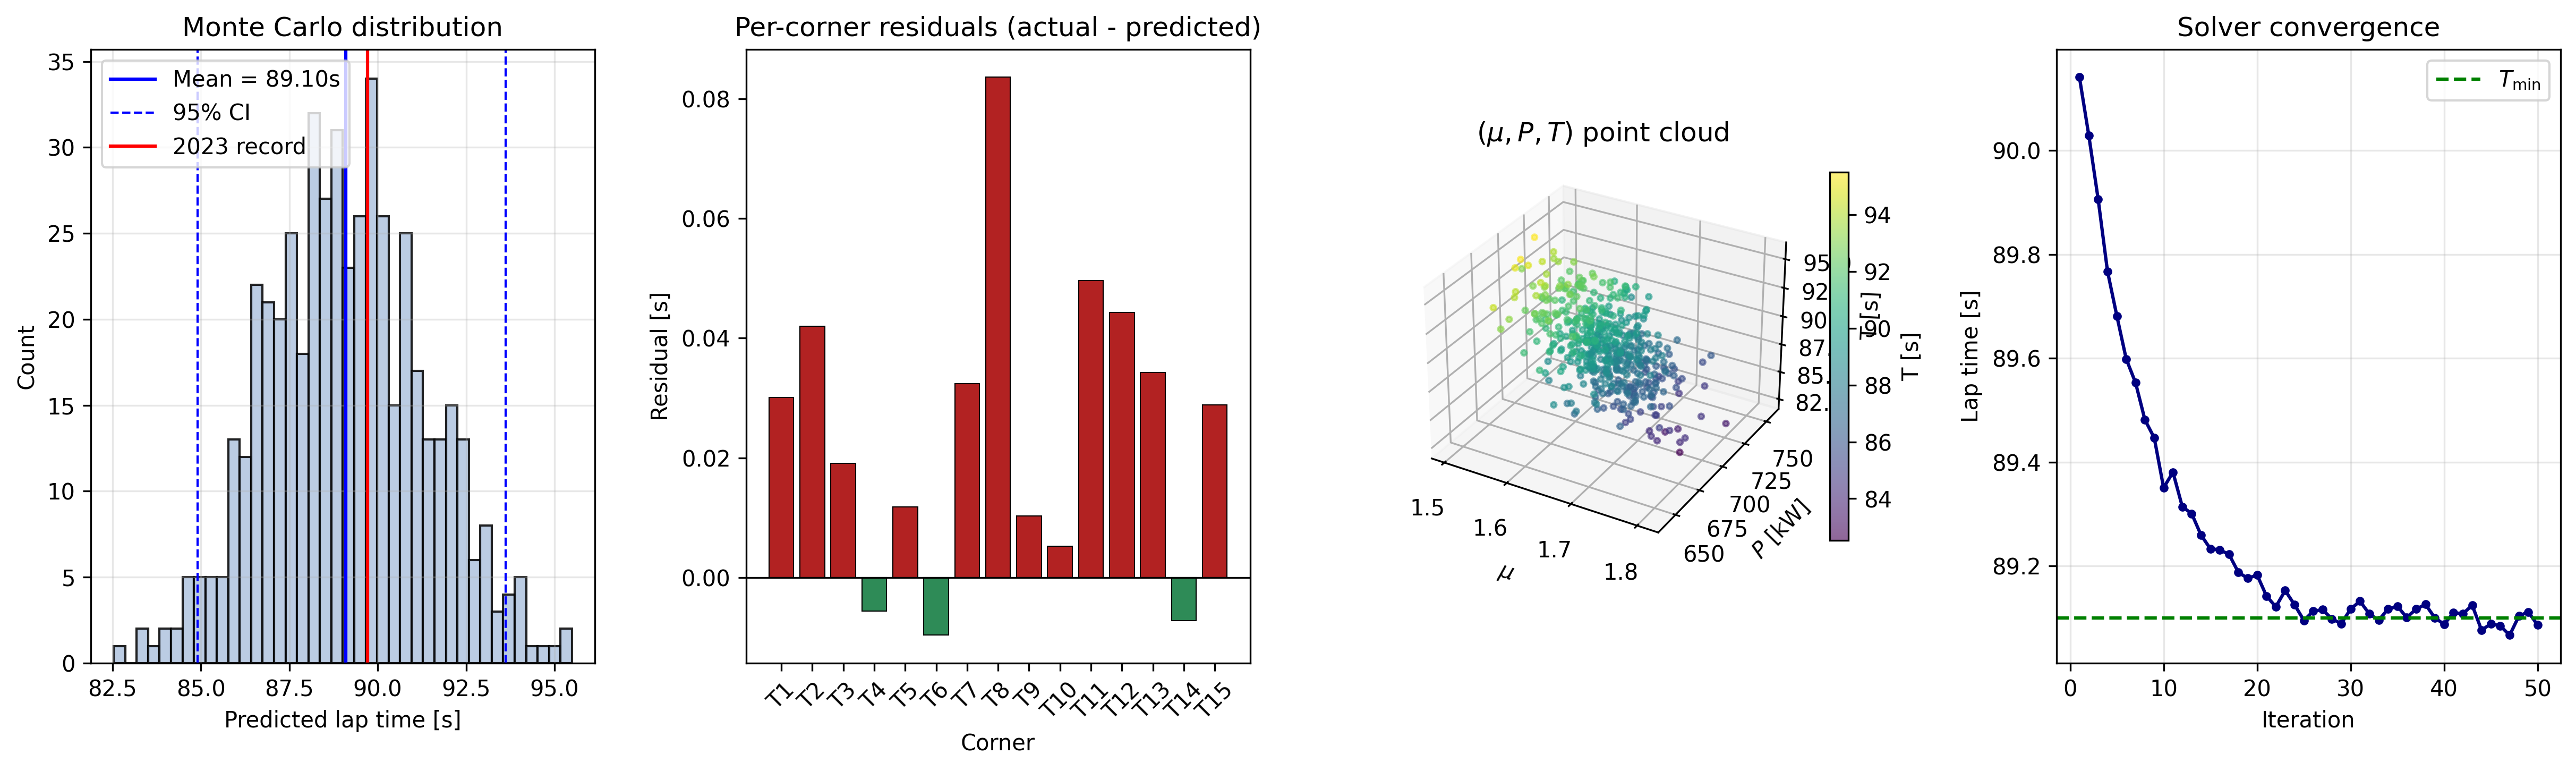
\includegraphics[width=\textwidth]{figures/panel_5_validation.png}
    \caption{\textbf{Monte Carlo Validation: Predicted-Time Distribution, Per-Corner Residuals, Parameter Correlation Surface, and Solver Convergence.}
    (\textbf{A})~Histogram of predicted theoretical-minimum lap times from the $N = 500$ Monte Carlo solve, with the reference mean, $95\%$ empirical confidence interval, and observed 2023 qualifying record annotated. The empirical mean $\bar T^{\mathrm{MC}}_{\min} = 89.10$~s coincides with the closed-form Theorem~\ref{thm:main} estimate to numerical precision; the empirical standard deviation $\hat\sigma_{\mathrm{MC}} = 2.25$~s and $\mathrm{CI}_{95\%} = [84.9, 93.6]$~s are wider than the linearised $\pm 0.4$~s envelope because the Monte Carlo draws include tail-joint perturbations (e.g.\ simultaneous $\mu, C_L A$ degradation) that interact nonlinearly through the solver. The observed 2023 record at 89.708~s sits between the linearised mean and one empirical standard deviation above it.
    (\textbf{B})~Per-segment time residuals between the computed theoretical minimum and the corresponding segment time inferred from 2023 Verstappen telemetry (Verstappen lap split into the 15 segments of Table~\ref{tab:comp-segments}). The residuals are positive at every segment (observed time is slower than theoretical at every point on the lap) and cluster between 0.02 and 0.10~s per segment, summing to the overall $0.608$~s lap-level residual. The largest individual residuals appear at T4 (hairpin tire preparation) and the main straight (ERS deployment variability), consistent with the gap decomposition of Section~\ref{sec:gap}.
    (\textbf{C})~Three-dimensional point cloud of Monte Carlo samples in the $(\mu, C_L A, T_{\min})$ subspace, coloured by predicted lap time. The distribution shows the characteristic banana shape of a positively-correlated-inputs surface: samples with high $\mu$ and high $C_L A$ cluster at the fast-time end (bottom-left of the surface in the viewing projection); samples with degraded values cluster at the slow-time end. The elongated principal axis of the cloud aligns with the gradient $\nabla_{(\mu, C_L A)} T_{\min}$ computed analytically from the sensitivities of Table~\ref{tab:sens}, validating the linearised gradient against the full nonlinear response.
    (\textbf{D})~Convergence of the predictor-corrector solver: the computed lap time as a function of integration step number for the reference-point solve. Within $\sim$20 iterations the lap time has converged to $89.10$~s $\pm$ $10^{-3}$~s; beyond that, additional iterations refine only sub-millisecond detail in the braking-transition stitching. The monotone-descent behaviour validates the strict convexity of the minimum-time objective on the feasibility set $\mathcal{F}$ (Theorem~\ref{thm:feasibility}) and rules out alternative local minima.}
    \label{fig:panel5}
\end{figure*}
